

\chapter{Using Deep Learning to Detect Technical Debt}

We aim to create a system that automatically detects technical debt in a class method. To achieve this goal, we took the following three steps: dataset creation, classification and hyperparameter tuning.
The dataset was automatically created by mining and processing open-source project histories. It's a balanced dataset by construction and the two classes are referred as: SATD and fixed.

We initially identify technical debt through the presence of SATD in the comments of the source code, using keyword labels pattern matching \cite{potdar2014exploratory} \cite{rantala2020prevalence}.
The identification of a SATD/fixed method pair is based on a strong assumption: when the SATD comment disappears, due to a commit, we suppose that the technical debt is fixed; so, we regard the new code as TD-free, i.e. belonging to fixed class.
% detail: describe the circumstances where we reject this hypotheses
The classifier is a neural network capable of representing snippets of code with an fixed length vector, conceptually similar on how word2vec works. The learned vector representation (code embedding) is associated with a semantic label (i.e. SATD or fixed).
Lastly, to increase the performance of the system we select a set of hyperparameters and perform a distributed grid search for tuning their values. The rest of this chapter explains each part in greater detail.

%3.1
\section{Mining SATD Instances and their Fixes}

These are the fundamental activities involved in the creation of the dataset:
\begin{itemize}
    \item Github repository url mining: using Github api, we extracted 248,872 projects' url matching our search profile.
    \item Repository cloning and filtering: some projects can be discarded only after the commit history is available for a precursory analysis to determine if a project qualifies for the next activity.
    \item Commit history processing: the directed acyclic graph of the commits is traversed and the source code is parsed in search of acceptable SATD/fixed pair.
\end{itemize}

The following sections describe these activities in detail.

\subsection{Github repository url mining}
We know from experience and from the literature that the concentration of SATD is very low \cite{bavota2016large} \cite{maldonado2015detecting} \cite{potdar2014exploratory}, for this reason we tasked ourselves to create a dataset from an initial set of open-source projects as big as possible. 
The search was conducted for all public Java GitHub repositories in a 20 years time window (from 2000 to 2019). 
The retrieval process of this URLs list was challenging in itself. We dealt and solved the following issues:
\begin{enumerate}
    \item GitHub search API limit of 1000 hits.
    \item GitHub search API number of request per minute maximum quota.
    \item Filtering to remove low quality repositories
\end{enumerate}
The first issue was solved with using two different phases of query: probe and search. The probe query requests only the number of the repositories that were created in a specific time window; if the number exceeds the 1000 limit, it iteratively divides the query in two sub-queries using half of the time window for each.
It was not enough to specify the day interval in the query; the time of the day was needed also because in the recent years there are multiple instances of more than 1000 repositories created in a single day.

The second issue was solved using an authentication token, as specified by the GitHub documentation.

The last issue was the reason we switched to the GitHub GraphQL API; we quickly realized that the total number of repositories in the selected period was more than seven millions and we needed a way to trim down the list to those most meaningful repositories. We empirically defined, through a trial and error process, a metric to keep those repositories with a good likelihood to contain \textit{higher quality source code}. 
The GraphQL Repository API can be queried to return additional information; for each repository, we requested the issue count and the commit count so to discard quickly those with less or equal than 100 commits and 100 issues.
The total number of URLs retrieved was roughly seven million but we did clone only a subset of them: around 250 thousand repositories.


% 6 47 57
% query range 20 anni, a lot of java projects
% github api v4, why?
% keep projects with issue count > 100 or commit count > 100
% token to use for speed
% save urls to text file
% total urls spooled 7 million
% that passed the 


% javaparser & pre-selection of repositories by api.


% Building a list of github repositories - github api tool -reject android repositories
% %mention the initial idea of specialization
% %remember --##string##--

% The process of cloning and caching repos.
% The source code processing. SATD search, exclusions, metrics (lines, tokens)
% Caching of code vectors.
% Parsing, comment cleaning, excluded patterns.
% SATD/fixed tracking. 
% Saving to h2 and then postgresql.

\subsection{Repository cloning and filtering}


\subsection{Commit history processing}
% the commit is like a function that transform the SATD in fixed
%3.2 
\section{The Deep Learning Model}
The model described in this section is called code2vec \cite{alon2019code2vec}.
The following three sequential processes can be considered a chain that progressively transform the source code into the desired target (i.e. the two classes SATD/fixed):
\begin{itemize}
    \item Decompose
    \item Aggregate
    \item Predict
\end{itemize}

\noindent Each of these steps can be viewed as a process that takes an input, creates an intermediate representation and generates an output for the next process.
In the rest of this section we give some details about each one of them and introduce some technical terms. 
\\
\\
\noindent \textbf{Decompose.} The input of this process is the source code. The output generated is a bag of path-context. The following list gives more detail on the process and the intermediate representations:

\begin{itemize}
    \item Parsing and creation of the abstract syntax tree of the method source code. 
    \item Extraction of all AST-paths (up to a fixed limit).
    \item Encoding of the AST-paths into a bag of context-vector.
    \item Transform each context-vector into a path-context (so to obtain a bag of path-context).
\end{itemize}

\noindent \textbf{Aggregate.} This process aggregates the bag of path-context (the output from the previous process) using an attention vector. The final result is a code-vector that represents the snippet of code as continuous distributed vector, i.e. a `code embedding'.
\\
\\
\noindent \textbf{Predict.} The code-vector is feeded to a fully connected neural network that performs the classification using the desired classes (i.e. SATD/fixed).
\\
\\
\noindent In the following sections we expand and dig deeper in these concepts.

% Here I want to explain briefly what are the fundamental pieces and how they interact (without pretending that the reader really understands, but to give the general idea)

\subsection{Representing code using AST-paths}
This section describes how to capture semantic information from a snippet of code and create a representation that can be used to predict properties of the snippet, for example a label (e.g. SATD/fixed).
To better illustrate how the decomposition is done, we use the simple code snippet in listing \ref{lst:snippet_ast_code} as an example .

%AST of code snippet
\begin{lstlisting}[caption={Example code to show decomposition}, label={lst:snippet_ast_code},language=Java]

                            String METHOD_NAME() {
                              if(somePreCondition())
                                while(!completed())
                                   doWork();
                              return "ok";
                            }
                            
\end{lstlisting}

Using JavaParser \footnote{https://javaparser.org/} the abstract syntax tree (AST) is extracted from the source code; see an example in figure  \ref{fig:AST_graphviz}.


\begin{figure}
 \centering
 \resizebox{\columnwidth}{!}{
 \includesvg[]{images/AST_graphviz}
 }
 \caption[AST for listing \ref{lst:snippet_ast_code}.]{Abstract syntax tree of the source code presented in listing \ref{lst:snippet_ast_code}.}
 \label{fig:AST_graphviz}
\end{figure}

	
We identify three sets of node in the AST: values, terminal and non-terminal nodes. Values are the leafs (this set is identified with $X$), terminal nodes are the immediate parent of a leaf and the rest are the non-terminal ones.
\textit{AST-path definition}: it is a path connecting two terminal nodes and it must include one non-terminal node which is a common ancestor of the two terminal nodes. 
The representation of the program is the \textit{set of all its AST-paths}. 

To wrap up this section, we explain the last AST-path in figure \ref{fig:AST_paths} and, for convenience, this AST-path is also reported here:

%AST-paths only last
\begin{center}
  \makebox[\textwidth]{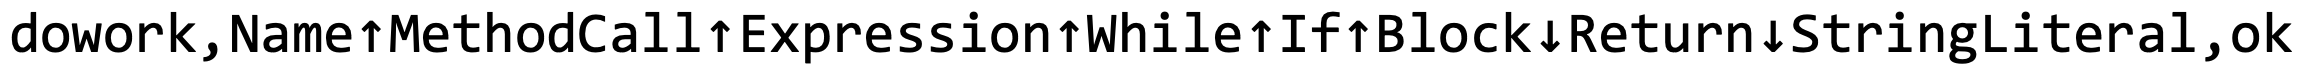
\includegraphics[width=\columnwidth]{images/AST_paths_last.png}}
\end{center}

The two value nodes are the first and the last words, `dowork' and `ok' respectively; the reader can also identify these leaf nodes in the bottom-right part of figure \ref{fig:AST_graphviz}.
The central part of the AST-path above is the connecting path between those two value nodes: it lists all the intermediate nodes and it also specifies the direction (up or down) one needs to take to traverse the tree. The common ancestor, for this example, is the intermediate node called `block'.

%AST-paths of code snippet
\begin{figure}
 \centering
 \resizebox{\columnwidth}{!}{
  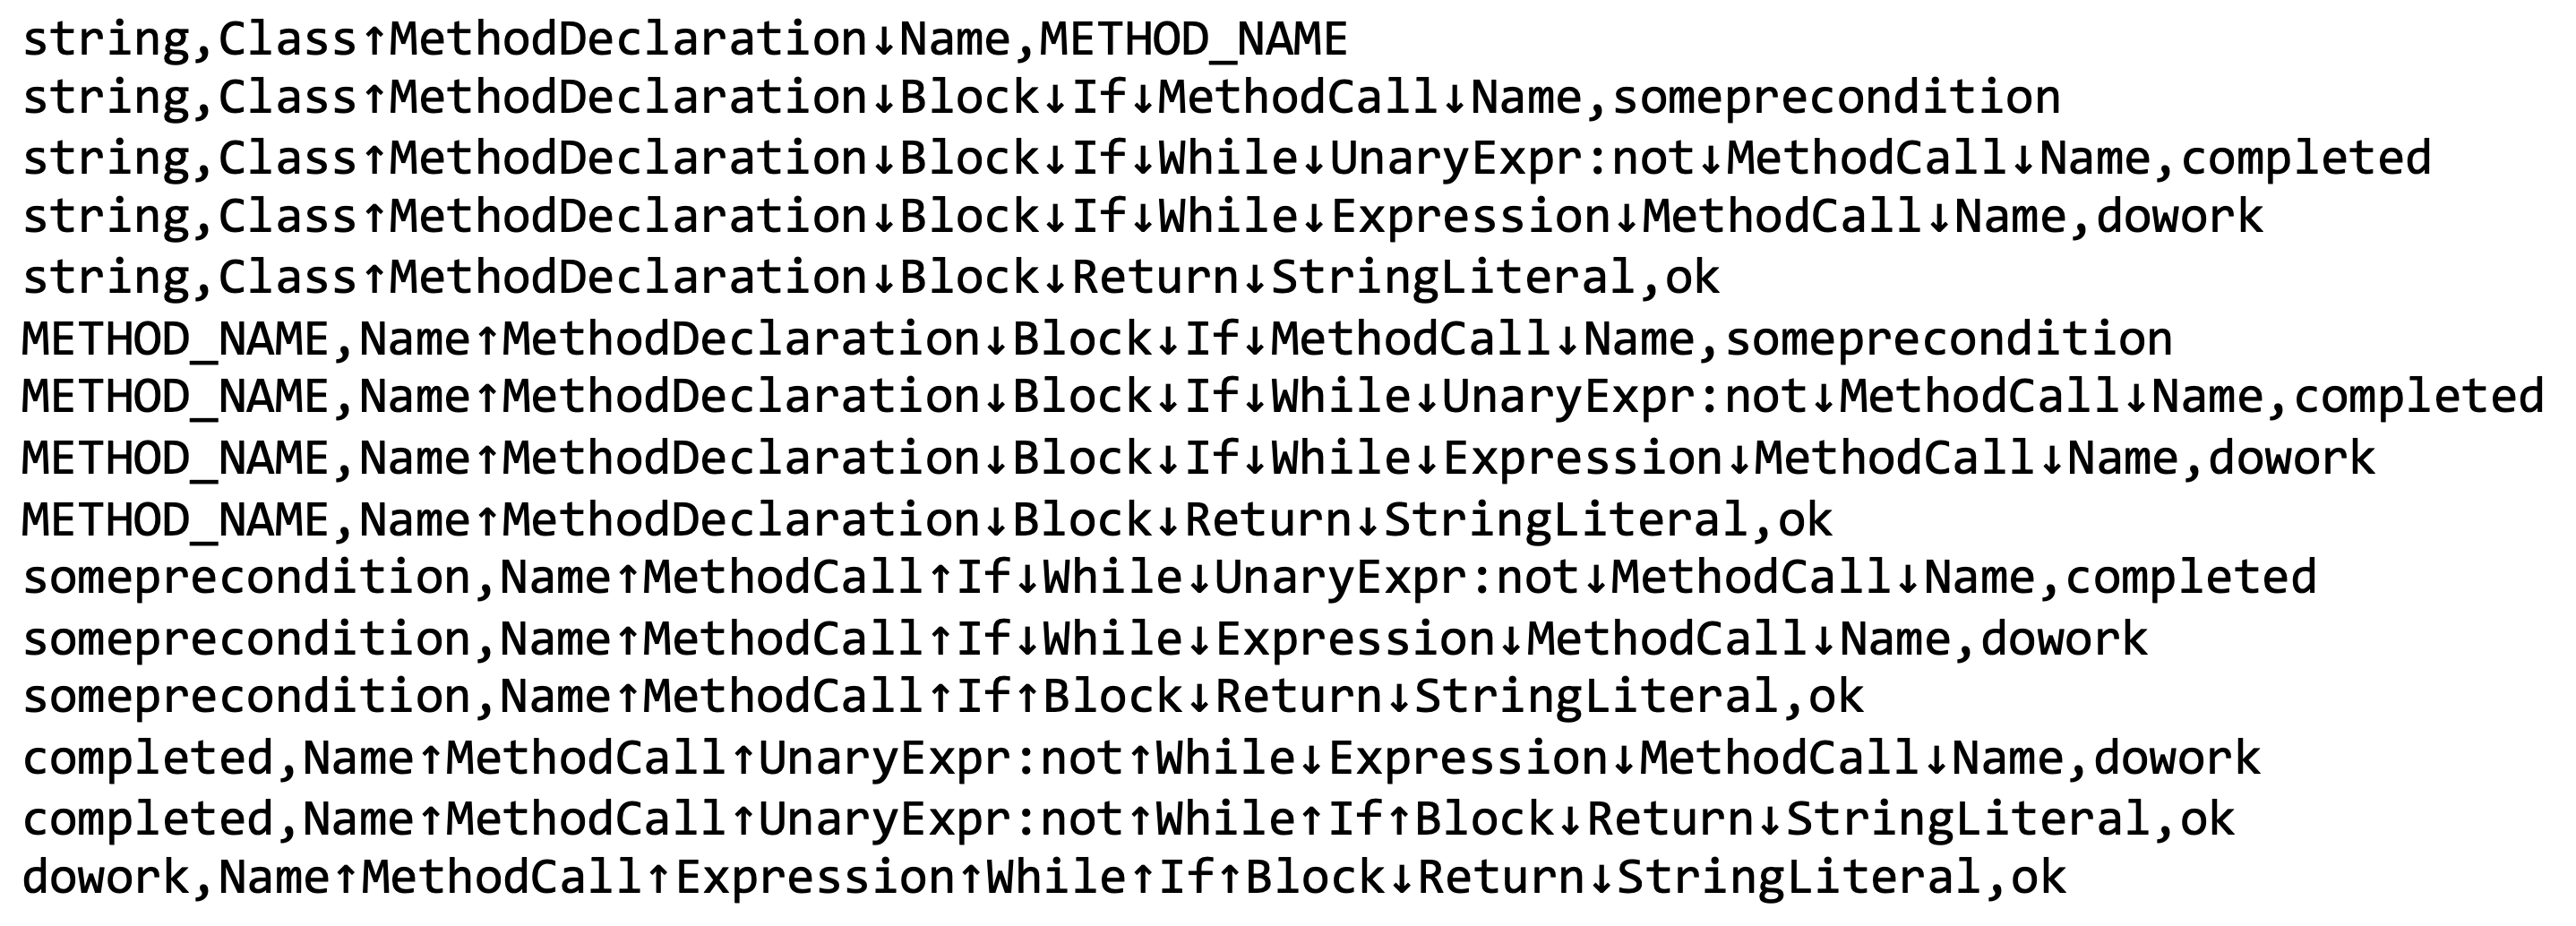
\includegraphics{images/AST_paths.png}
 }
 \caption[All AST-paths for listing \ref{lst:snippet_ast_code}.]{AST-paths of listing \ref{lst:snippet_ast_code}.}
    \label{fig:AST_paths}
\end{figure}

% here I go into details on the first decomposition/representation of the code snippets into fixed length vectors

What is seen in figure \ref{fig:AST_paths} is a bag of context-paths (another name for the set of all AST-paths) and it is the representation for the code snippet. The following section explains how these AST-paths are transformed into fixed length vectors.

\subsection{Context-vector}
%how many OOV? 
%https://github.com/tech-srl/code2vec/blob/c98e8f786b7262e56c93e520d039fb7aa5d0f7ef/vocabularies.py#L123

A context-vector $c_i$ is the vector representation for one AST-path. The process of transformation is applied to all AST-paths producing a bag of context-vectors.
The following picture shows how the context-vector is formed:

\begin{center}
  \makebox[\textwidth]{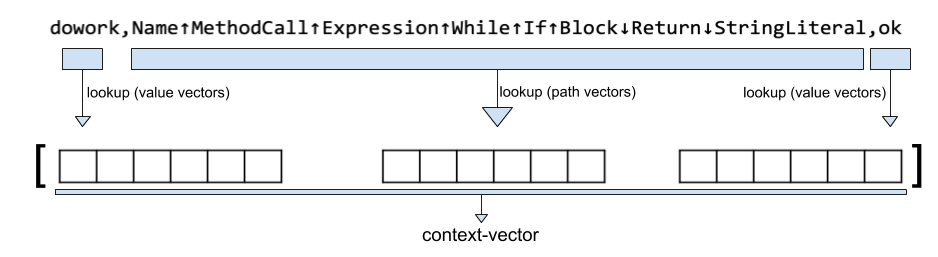
\includegraphics[width=\columnwidth]{images/context_vector.png}}
\end{center}

To explain the picture above we need to introduce two matrices:
\begin{align*} 
 value\_vocab \in \mathbb{R}^{|X| \times d}
\\
    path\_vocab \in \mathbb{R}^{|P| \times d}
\end{align*}
% \begin{itemize}
%     \item value\_vocab $\in \mathbb{R}^{|X| \times d}$
%     \item path\_vocab $\in \mathbb{R}^{|P| \times d}$
% \end{itemize}

The embedding size $d$ is an hyperparameter. $X$ is the set of values of the AST terminals that were observed during training; in our recurring example this set is composed by: string, METHOD\_NAME, someprecondition, completed, dowork and ok. 
$P$ is the set of all AST-paths across all snippets.

These matrices are initialized randomly and are learned by the model during the training.
An embedding (either from value\_vocab or path\_vocab) is looked up selecting the appropriate row in its matrix.

The previous notions tells us that:
\begin{align*} 
c_i \in  \mathbb{R}^{3 d}
\end{align*}

The two matrices value\_vocab and path\_vocab do not need to be of the same width $d$ but for convenience it was chosen so.

\subsection{Path-context}
The previous section describes the definition of the context-vector $c_i$. Applying a fully connected layer to it we obtain the path-contest vector $\widetilde{c}_i$, also called combined context-vector. The following equation describes the computation of this layer:

\begin{align*} 
\widetilde{c}_i = \tanh( W \cdot c_i )
\end{align*}
where $W$ is the weight matrix and
\begin{align*} 
W \in  \mathbb{R}^{d \times 3 d}
\end{align*}

The height of $W$ is for convenience of the same size as before ($d$); it does not need to be strictly so: it can also be of different height.
One other way to look at this layer is that it compresses the context-vector $c_i$ of size $3d$ into a combined context-vector of size $d$.

\subsection{Attention mechanism and the code-vector}

The previous section left us with a set of path-contexts. The goal of this part of the model is to combine them all into a code-vector.
This step employs an attention vector $a$.
\\
\noindent \emph{-- stopping until feedback on this section --}

 

\subsection{Training and prediction}
% detailed explanations in step:
% - representation idea (ast, path learning)

% - semantic labeling

% - SATD/fixed

% The model used is called code2vec. The idea is to represents source code snippets using a fixed length vector i.e. code embedding. 
% The abstract syntax tree (AST) is used, there is an attention mechanism and it was successful in predicting semantic labeling.

% Simple and fast


%3.3
\section{Hyperparameter Tuning}

This section describes the process of tuning the hyperparameters of the model.

It is clear that using shorter code snippets increases the performance but decreases the number of samples in the dataset; thus decreasing the usefulness of the trained model because of less capability in generalization.
For the tuning of the hyperparameters, we empirically defined to keep those snippets with less than 200 tokens; an example of a method composed by 199 tokens is shown in listing \ref{lst:snippet199}.

\begin{lstlisting}[caption={Code snippet with 199 tokens}, label={lst:snippet199},language=Java]
private CompoundWorkflow finishCompoundWorkflow(
  WorkflowEventQueue queue,
  CompoundWorkflow compoundWorkflow, 
  String taskOutcomeLabelId, 
  String userTaskComment, 
  boolean finishOnRegisterDocument, 
  List<NodeRef> excludedNodeRefs) {
    if ((finishOnRegisterDocument &&
      compoundWorkflow.isStatus(Status.FINISHED)) ||
      (!finishOnRegisterDocument &&
      checkCompoundWorkflow(compoundWorkflow,
      Status.IN_PROGRESS, 
      Status.FINISHED) == Status.FINISHED)) {
        if (log.isDebugEnabled()) {
            log.debug("--##string##--" + compoundWorkflow);
        }
    } else {
        setWorkflowsAndTasksFinished(queue, compoundWorkflow, 
            taskOutcomeLabelId, userTaskComment,
            finishOnRegisterDocument, excludedNodeRefs);
        if (finishOnRegisterDocument || excludedNodeRefs != null) {
            stepAndCheck(queue, compoundWorkflow);
        } else {
            stepAndCheck(queue, compoundWorkflow, Status.FINISHED);
        }
        boolean changed = saveCompoundWorkflow(queue,
            compoundWorkflow, null);
        if (log.isDebugEnabled()) {
            log.debug("--##string##--" + compoundWorkflow);
        }
    }
    CompoundWorkflow freshCompoundWorkflow =
        getCompoundWorkflow(compoundWorkflow.getNodeRef());
        
    if (!finishOnRegisterDocument && excludedNodeRefs == null) {
        checkCompoundWorkflow(freshCompoundWorkflow, Status.FINISHED);
    }
    checkActiveResponsibleAssignmentTasks(
        freshCompoundWorkflow.getParent());
    return freshCompoundWorkflow;
}
\end{lstlisting}

\noindent \emph{-- Expand the following paragraph with more detail and graphs) --}

We inspected all the hyperparameters and set up a grid search using a tools called Optuna.
The hyperparameters subject of the distributed experiment are: embedding size, dropout keep rate and context length.
We run it with multiple GPU colab PROfessional and standards sessions. Both cpu and GPU. 

